\documentclass[12pt,a4paper]{article}
\usepackage[utf8]{inputenc}
\usepackage{fontenc}
\usepackage{xcolor}
\usepackage{amsmath}
\usepackage{amsfonts}
\usepackage{amssymb}
\usepackage[spanish,es-tabla]{babel}
\usepackage{anysize}
\usepackage{setspace}
\usepackage{hyperref}
\usepackage{graphicx}
\usepackage{float}
\usepackage{subfigure}
\usepackage{multicol}
\usepackage{fancyhdr}
\marginsize{3.50cm}{2.50cm}{3.00cm}{3.00cm}
\setlength{\parindent}{8mm}
\doublespace



\title{Taller de \LaTeX}
\author{Autor 1\and Autor 2}
\date{\today}

%Modificación de las enumeraciones
\renewcommand{\theenumi}{\arabic{enumi}}
\renewcommand{\theenumii}{\Alph{enumii}}
\renewcommand{\theenumiii}{\alph{enumiii}}
\renewcommand{\theenumiv}{\roman{enumiv}}

\renewcommand{\labelenumi}{{\theenumi}.}
\renewcommand{\labelenumii}{{\theenumii}.}
\renewcommand{\labelenumiii}{{\theenumiii})}
\renewcommand{\labelenumiv}{{\theenumiv}.}

%colores
\definecolor{titulos}{rgb}{0.5, 0.0, 0.0}

%Instrucciones para las columnass
\setlength{\columnsep}{0.7cm} %La separacion de las columnas
\setlength{\columnseprule}{1pt} %Dibuja una linea entre las columnas
\def\columnseprulecolor{\color{titulos}}

%Personalizacion del documento
\fancyhead[L]{Dinámica No Lineal}
\fancyhead[C]{}
\fancyhead[R]{\leftmark}
\fancyfoot[L]{Informe N°1}
\fancyfoot[C]{\thepage}
\fancyfoot[R]{Flores Q., F.}

\renewcommand{\headrulewidth}{2pt}
\renewcommand{\footrulewidth}{2pt}

%Caratula
\fancypagestyle{plain}{
\fancyhead[L]{}
\fancyhead[C]{}
\fancyhead[R]{}
\fancyfoot[L]{}
\fancyfoot[C]{}
\fancyfoot[R]{}

\renewcommand{\headrulewidth}{0pt}
\renewcommand{\footrulewidth}{0pt}
}

\pagestyle{fancy}
\begin{document}
\maketitle
\newpage

\tableofcontents
\newpage
\begin{abstract}
La mecánica cuántica a la rama de la física contemporánea dedicada al estudio de los objetos y fuerzas de muy pequeña escala espacial, es decir, de la materia a nivel del átomo y de las partículas que lo componen, así como los movimientos que las caracterizan.
\end{abstract}
\renewcommand{\abstractname}{Abstract}
\begin{abstract}
Quantum mechanics is the branch of contemporary physics dedicated to the study of objects and forces of very small spatial scale, that is, matter at the level of the atom and the particles that compose it, as well as the movements that characterize them.
\end{abstract}

\part{Introducción al \LaTeX}
\section{Escritura}\label{introduccion}
La teoría de la relatividad especial, también llamada teoria de la\linebreak relatividad restringida, es una teoría de la física publicada en 1905 por Albert Einstein. Surge de la observación de que la velocidad de la luz en el vacío es igual en todos los sistemas de referencia inerciales y de obtener todas las consecuencias del principio de {\it \large relatividad de Galileo}.
\section{Relatividad}
Según el, cualquier experimento realizado en un sistema de {\sc referencia} \linebreak {\sc inercial} se desarrollara de manera idéntica en cualquier otro sistema inercial. Información que aparecerá en la página.\begin{enumerate}
\item Primera sesión de \LaTeX.
\item Semana libre
\item Segunda sesión de \LaTeX.\begin{enumerate}
	\item Primera sesión de \LaTeX.
	\item Segunda sesión de \LaTeX.\begin{enumerate}
	\item Primera sesión de \LaTeX.
	\item Segunda sesión de \LaTeX.\begin{enumerate}
	\item Primera sesión de \LaTeX.
	\item Segunda sesión de \LaTeX.
	\item Tercer sesión de \LaTeX.
\end{enumerate}
	\item Tercer sesión de \LaTeX.
\end{enumerate}
	\item Tercer sesión de \LaTeX.
\end{enumerate}
\item Tercer sesión de \LaTeX.
\end{enumerate}

\begin{itemize}
	\item Primera sesión de \LaTeX.
	\item Señale verdadero o falso.\begin{itemize}
	\item Primer enunciado
	\item[$\star$] Segundo enunciado
	\item Tercer enunciado
	\end{itemize}
	\item Tercer sesión de \LaTeX.
\end{itemize}

Tengo 35 \$, $\o$
 
$$P=50\,\textsc{atm}$$

\begin{equation}
\label{Atmos}
P=50~\text{atm}
\end{equation}

\subsection{Tipos de escritura}
\subsubsection*{Párrafo}

\begin{itemize}
\item Si yo uso \texttt{textbf}\{\text{texto}\}, lo que este dentro se pondrá en negrita:\\``\textbf{texto}''

\item Si yo uso \texttt{textit}\{\text{texto}\}, lo que este dentro se pondrá en cursiva:\\``\textit{texto}''

\item Si yo uso \texttt{textsc}\{\text{texto}\}, lo que este dentro se pondrá todo en\linebreak mayuscula:\\``\textsc{texto}''

\item Si yo uso \texttt{textsf}\{\text{texto}\}, lo que este dentro se pondrá todo en\linebreak mayuscula:\\``\textsf{texto}''

\item Si yo uso \texttt{textsl}\{\text{texto}\}, lo que este dentro se pondrá todo~en~mayuscula~ss:\\``\textsl{texto}''

\end{itemize}

\subsection*{Escritura de formulas}\label{formulas}
Existen tres formas de escribir formulas:\begin{itemize}
\item \textbf{Escritura lineal}: Para ello solamente se deben utilizan un símbolo de dolar en cada extremo (\$).\begin{center}
Ella no te ama $m=\cfrac{y_2-y_1}{x_2-x_1}$, me fue infiel
\end{center}


\item \textbf{Escritura centrada}: Para ello se deben utilizan doble símbolo de dolar en cada extremo (\$\$).\\[0.2cm]
No olvidar que la función de onda se escribe: $$\Psi(r,\theta,\phi)=R(r)\Theta (\theta,\phi)$$ La parte angular tiene solución con \textbf{armónicos esféricos}

\item \textbf{Escritura enumerada}: Para ello debemos usar el comando \texttt{begin}\{\text{equation}\}\\[0.2cm]
Según $\cdots$, la ecuación fundamental de la termodinámica es:\begin{equation}
T\text{d}S=\text{d}U+p\text{d}V-\mu\text{d}N
\end{equation}
$$\text{d}S=\frac{\text{d}U}{T}+\frac{p\text{d}V}{T}-\frac{\mu\text{d}N}{T}$$
\end{itemize}

\section{Matrices}\label{matriz}
Segun De La Peña \cite{DLP} y Muñoz \cite{MJM}
\subsection*{Vectores}
$$\vec{v}=\textbf{v}=\begin{pmatrix}
a_{11} \\ a_{12} \\ a_{13} \\ \vdots \\ a_{1n}
\end{pmatrix}$$

$$\vec{v}=\textbf{v}=\begin{vmatrix}
a_{11} \\ a_{12} \\ a_{13} \\ \vdots \\ a_{1n}
\end{vmatrix}$$

\subsection*{Matrices}
$$A=\begin{pmatrix}
a_{11} & a_{21} & a_{31} & \hdots & a_{m1} \\
a_{12} & a_{22} & a_{32} & \hdots & a_{m2} \\
a_{13} \\
\vdots \\
a_{1n}
\end{pmatrix}$$

Como se pudo ver en la pagina \pageref{formulas} indicamos las formas es escribir las ecuaciones. Y la solución final la pudimos ver en la pagina \pageref{Atmos}. La lista de asistencia aparece \href{https://forms.gle/84VyN2QJq7twTHH87}{haciendo click aqui}

\newpage
\part{Teoría del Caos}
\section{Atractor de Lorentz}
Como una cuestión previa conviene aclarar conceptos porque tiende a confundirse Caos y Fractales (ver figura \ref{img:fibo}). En artículos de divulgación y en muchas publicaciones vienen juntos y mezclados, por lo que hay que precisar que Caos y Fractales no son sinónimos y tienen comportamientos distintos a pesar de compartir una formulación sencilla y que ciertos fenómenos caóticos tengan una estructura fractal como es el caso del atractor de Lorenz que podemos observar en la figura \ref{img-lorentz} visto en la pagina \pageref{img-lorentz}.
\begin{figure}[H]
	\centering
	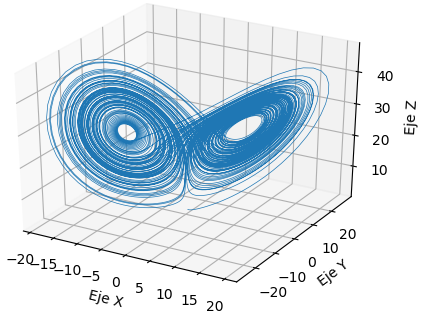
\includegraphics[scale=0.8]{img/tlorentz}
	\caption{Atractor de Lorentz}
	\label{img-lorentz}
\end{figure}
Los estudios de Edward Lorenz sobre  "Dependencia sensitiva de las condiciones iniciales" y el famoso efecto mariposa son el origen de la Teoría del Caos.
\begin{figure}[H]
	\centering
	\caption{Fractal de Fibonacci. Fuente: \url{https://rosettacode.org/wiki/Fibonacci_word/fractal}}
	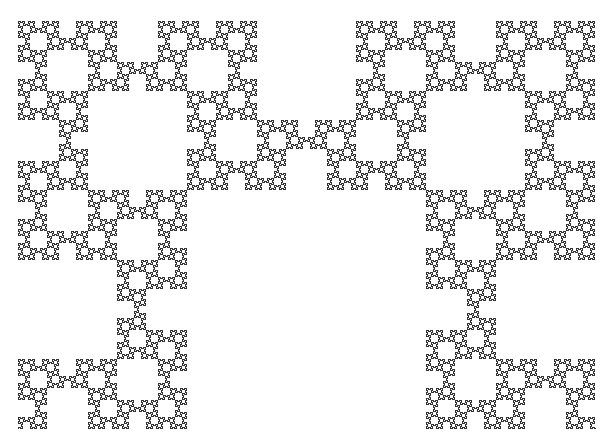
\includegraphics[scale=0.6]{img/fractal}
	\label{img:fibo}
\end{figure}
El término atractor extraño se debe a David Ruelle y Floris Takens, físico-matemático el primero y matemático el segundo. Lo definieron como: una zona bien delimitada del espacio de fases en la que las líneas de la trayectoria del sistema nunca se cortan. Líneas de longitud infinita confinadas en área finita, describiendo órbitas no periódicas. Ni Ruelle ni Takens lo habían visto nunca, pero presagiaron su existencia. Ese monstruo matemático, según ellos, debería de ser fractal.

\begin{figure}[H]
	\centering
	\subfigure[Primera figura]{
		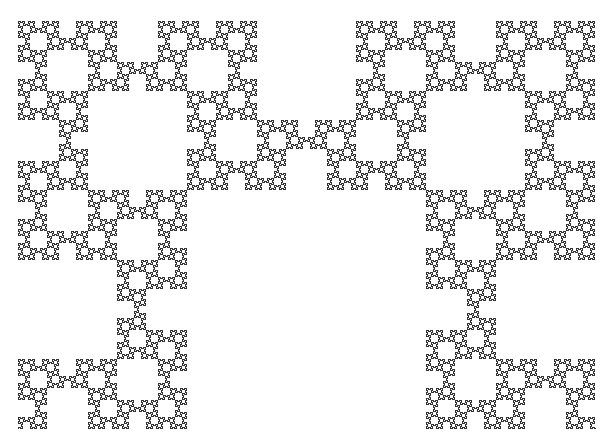
\includegraphics[scale=0.3]{img/fractal}}
		\quad
	\subfigure[Segunda figura]{
		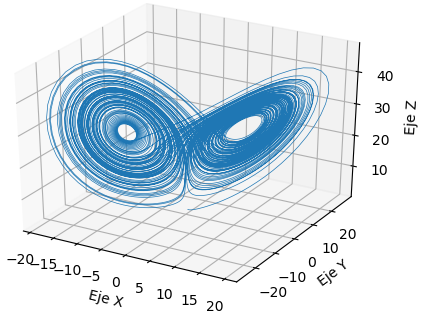
\includegraphics[scale=0.4]{img/tlorentz}}
	\caption{Gráficas importantes en la teoria del caos}
\end{figure}

Sea la tabla \ref{tb:implementos} podemos observar los implementos necesarios para poder restaurar nuestro laboratorio de Química General.

\begin{table}[h]
\begin{center}
\caption{}
	\begin{tabular}{| c | c | c | c |}
		\hline
		\multicolumn{4}{| c |}{Instrumentos} \\ \hline
		\multicolumn{2}{| c |}{Items} & \multicolumn{2}{| c |}{Inventario} \\ \hline
		\bf Materiales & \bf Precio & \bf Cantidad & \bf Salón \\ \hline
		Probeta & 70 & 5 & KFC-1\\
		Matraz & 26 & 13 & KFC-2\\
		Pipeta & 30 & 3 & KFC-3\\ \hline
	\end{tabular}\\
	\normalsize{Implementos para un laboratorio de Química I}
	\label{tb:implementos}
\end{center}
\end{table}

\section{Exponente de Lyapunov}
\begin{multicols}{2}
El Exponente Lyapunov o Exponente característico Lyapunov de un sistema dinámico es una cantidad que caracteriza el grado de separación de dos trayectorias infinitesimalmente cercanas. Cuantitativamente, dos trayectorias en el espacio-fase con separación inicial $\delta Z_0$ diverge.

El radio de separación puede ser distinto para diferentes orientaciones del vector de separación inicial.\columnbreak

Aunque, hay un completo espectro del exponente Lyapunov; el número de ellos es igual al número de dimensiones del espacio-fase. Es común referirse sólo a la más grande, porque determina la predictibilidad de un sistema.
Los exponentes característicos de Lyapunov (LCE del inglés Lyapunov Characteristic Exponents) son una herramienta que permite cuantificar la velocidad a la que se separan dos órbitas con condiciones iniciales infinitamente cercanas. Por ello, con frecuencia se emplean como indicadores de la presencia de caos.
\end{multicols}


\newpage
\renewcommand{\refname}{Bibliografía}
\begin{thebibliography}{2}
\bibitem{DLP} De La Peña, L. (2014). Introducción a la mecánica cuántica. Fondo de Cultura económica.
\bibitem{MJM} Muñoz, J. M. (2015). Mecánica cuántica y libre albedrío: cinco cuestiones fundamentales. Principia: an international journal of epistemology, 19(1), 65-92.
\end{thebibliography}



\end{document}
